\documentclass[12pt,a4paper]{article}
\usepackage[utf8]{inputenc}
\usepackage[T1]{fontenc} 
\usepackage[french]{babel}
\usepackage{fullpage}
\usepackage{amsmath}
\usepackage{amsfonts}
\usepackage{amssymb}
\usepackage{color}
\usepackage{titlesec}
\usepackage{indentfirst}
\usepackage[french]{varioref}
\usepackage{graphicx}
\usepackage{subfig}
\usepackage{tocloft}
\usepackage[backend=bibtex,bibstyle=authoryear]{biblatex}
\usepackage{url}
\usepackage{natbib}

% Aerer les tableaux
\renewcommand{\arraystretch}{1.5}
\setlength{\tabcolsep}{0.5cm}

\makeatletter
\definecolor{vert}{rgb}{0,0.5,0}
\definecolor{vertclair}{rgb}{0.85,1,0.85}
\definecolor{redclair}{rgb}{1,0.9,0.75}

\titleformat*{\section}{\color{red}\scshape\bfseries\LARGE}
\titleformat*{\subsection}{\scshape\bfseries\large}
\titleformat*{\subsubsection}{\normalsize\bfseries}

\titlespacing*{\section}{0cm}{0.5cm}{0.5cm}
\titlespacing*{\subsection}{1cm}{0.5cm}{0.3cm}
\titlespacing*{\subsubsection}{1.75cm}{0.3cm}{0.3cm}

\renewcommand{\thesection}{\textcolor{red}{\Roman{section}}}
\renewcommand{\thesubsection}{\textcolor{blue}{\Alph{subsection}}}
\renewcommand{\thesubsubsection}{\textcolor{vert}{\arabic{subsubsection}}}

\newcommand{\mnp}[1]{\mathcal{M}_{n,p}\left(\mathbb{#1}\right)}

% Le vocabulaire
\newcommand{\vocabulaire}[1]{\\ \begin{minipage}{1\textwidth}\textbf{Vocabulaire :} \begin{center}\begin{minipage}{0.8\textwidth}
        #1
      \end{minipage}\end{center}\end{minipage}}

% les théorèmes
\newtheorem{thm}{\textsc{Théorème}}
\newcommand{\theoreme}[2]{
  \begin{center}
    \fcolorbox{red}{redclair}{
      \begin{minipage}{0.9\textwidth}
        \begin{thm}[\emph{#1}] \color{red} \ \newline
              #2
        \end{thm}
      \end{minipage}}
  \end{center}}

% Résultat important
\newcommand{\important}[1]{
  \vskip 0.5cm
  \fcolorbox{red}{white}{
    \begin{minipage}[c]{0.9\linewidth}
      #1
    \end{minipage}
  }
  \vskip 0.5cm
}

% Les remarques
\newtheorem{rmq}{Remarque}
\newcommand{\remarque}[1]{
  \fcolorbox{black}{white}{
    \begin{minipage}{1\textwidth}
      \begin{rmq}
        #1
      \end{rmq}
    \end{minipage}}\smallskip}

% Les lemmes
\newtheorem{lem}{\textsc{Lemme}}
\newcommand{\lemme}[2]{
  \begin{center}
    \fcolorbox{red}{white}{
      \begin{minipage}{0.9\textwidth}
        \begin{lem}
          \label{#1}
          \textcolor{red}{#2}
        \end{lem}
      \end{minipage}}
  \end{center}\smallskip}

% Les preuves
\newcounter{pr}
\newcommand{\preuve}[3]{
  \addtocounter{pr}{1}
  \begin{center}
    \begin{minipage}{0.6\textwidth}
      \begin{center}
        \textbf{Démonstration \thepr \enspace-- #2 \ref{#1}}
      \end{center}
      #3
    \end{minipage}
  \end{center}\smallskip}

% cas 1,2...
\newlength{\caslength}
\newcommand{\cas}[2]{
  \begin{flushright}
    \begin{minipage}{0.9\textwidth}
      \settowidth{\caslength}{Cas #1 : }
      \parbox[b]{\caslength}{\textbf{Cas #1 :}}
      \parbox[t]{0.8\textwidth}{#2}
    \end{minipage}
  \end{flushright}
}

% méthode
\newsavebox{\methodebox}
\newenvironment{methode}[1]
{\small\savebox{\methodebox}{\textsc{Méthode : #1 }}\usebox{\methodebox}\\
  \begin{tabular}{rl}}
  {\normalsize\end{tabular}}

\newtheorem{exempletheoreme}{\textbf{Exemple}}
\newenvironment{exemple}{
  \begin{exempletheoreme}\normalfont \
    \begin{center}
      \begin{minipage}{0.9\textwidth}}
      {\end{minipage}
    \end{center}
  \end{exempletheoreme}
}


% les définitions
\newtheorem{definitiontheoreme}{\textbf{Définition}}
\newcommand{\definition}[2]{
  \begin{center}
    \fcolorbox{vert}{vertclair}{
      \begin{minipage}{1\textwidth}
        \begin{definitiontheoreme} \normalfont (\emph{#1}) \color{vert} \newline
          #2
        \end{definitiontheoreme}
      \end{minipage}}
  \end{center}}

\usepackage{minted}
\usepackage{verbatim}
\usepackage{moreverb}

\bibliography{bibliography}{}

\let\verbatiminput=\verbatimtabinput
\everymath{\displaystyle}
\addtolength{\textheight}{1cm}

\setlength{\cftsecnumwidth}{3em}
\setlength{\cftsubsubsecnumwidth}{2em}

\makeindex
\begin{document}
\thispagestyle{empty}
\begin{minipage}{1\textwidth}
  \centering 

  \begin{flushleft}
    
\includegraphics[scale=0.3]{LogoSup.jpg}
    \newline

    \textbf{Supélec - Campus de Metz\\
      $1^{ère}$ année - Année 2012-2013}\\
    \textsc{Le 14 Juin 2013}
  \end{flushleft}
  
  \vskip 5cm
  {\LARGE\textsc Soutenance de projet de synthèse}
  \vskip 0.5cm
  {\LARGE\textsc Création d'une ontologie à l'aide du logiciel Protégé}
  \vskip 5cm

  \Large{Alexandre Careil \\
    Thomas Bouchet}
\end{minipage}

\thispagestyle{empty}
\newpage
\null
\thispagestyle{empty}
\newpage 

\tableofcontents
\thispagestyle{empty}
\newpage

\thispagestyle{empty}
\null
\newpage

\listoffigures
\listoftables
\thispagestyle{empty}
\newpage

\thispagestyle{empty}
\null
\newpage

% Introduction
\section{Introduction}

\par Le technologies d'aujourd'hui permettent de stocker toujours plus de données, pour des coûts raisonnables. Il y a encore quelques années, les volumes échangés étaient limités par la vitesse de transmission et la capacité de stockage des médias disponibles. Ces contraintes ayant été outrepassées, l'accumulation de données est désormais telle qu'il devient difficile de les utiliser telles quelles. \emph{Big Data}, en Fran\c cais les \emph{Grandes Données} est le terme désignant cette masse conséquente, et englobe même tous les défis qui y sont liés, parmi lesquels l'analyse, la capture et le stockage.
\par Un des défis est justement d'appliquer des algorithmes sur ces données, mais de manière intelligente. Il ne s'agit pas en effet de considérer un seul ordinateur pour effectuer des calculs aussi conséquents, mais plutôt de répartir le traitement en plusieurs sous taches assignées à plusieurs unités de calcul indépendantes. De cette manière, au lieu de se limiter à la puissance d'une seule unité, on considère l'ensemble des ressources disponibles sur le réseau.
\par Des couches destinées à la gestion des ressources disponibles existent, et \emph{OAR} en fait partie. Elles permettent notamment de vérifier leur disponibilité et d'y lancer des traitements. Cependant, un problème majeur se pose : la difficulté de prise en main de cet environnement par n'importe qui. En effet, l'utilisation de cet environnement fait appel au \emph{shell} et nécessite l'apprentissage de commandes spécifiques. Notre but sera ainsi de fournir une surcouche logicielle permettant d'interagir avec les ressources disponibles sur le réseau à l'aide d'\emph{OAR} de manière transparente, et d'y lancer des taches pour traiter de gros fichiers de données et ainsi élargir le cercle des utilisateurs.

%%% Local Variables: 
%%% mode: latex
%%% TeX-master: "CompteRendu"
%%% End: 


% Description du projet
\section{Description du projet}

\par Le monde de l'IT fait actuellement parlé de lui à travers le Big Data. Google Trends rend compte de l'explosion de l'emploi de ce terme depuis fin 2010. Mais concrètement, quelle est l'utilité de ces technologies \emph{Big Data} dont tout le monde parle ? Les données produites par chacun au jour le jour représentent le nouvel Eldorado des sociétés qui voient en ces données l'occasion d'optimiser les process, d'améliorer l'expérience utilisateur, de proposer de nouveaux services ou encore, à titre d'exemple, d'aider la police à traquer les délinquants (\emph{L.A.}, \emp{USA}). Les applications \emph{Big Data} sont nombreuses et s'appuient pour partie sur les données open source mises en ligne par les gouvernements, les entreprises et les particuliers.

\par La deuxième année d'études à Supélec est ponctuée par la réalisation d'un projet de développement logiciel et d'un projet de conception chacun d'une durée d'une séquence (une année académique de Supélec est composée de quatre séquences).

\par Le choix des sujets est libre. C'est pourquoi nous avons choisi de nous intéresser aux technologies \emph{Big Data} et plus particulièrement à l'environnement Hadoop. Cet outil, très en vogue actuellement dans le monde de l'IT apparaît comme la référence dans le domaine.

\par Compte tenu de nos ambitions personnelles, notre projet prendra la forme d'un projet long, s'étalant donc sur deux séquences, et chapeauté par Mr Stéphane Vialle, professeur en Informatique à Supélec.

\par Notre projet s'articule en deux grandes parties. Premièrement, il s'agit d'une part de coder une interface graphique utilisateur en \emph{Java} à travers laquelle un utilisateur est en mesure de se connecter aux serveurs de Supélec ; d'autre part, il s'agit de permettre à l'utilisateur d'allouer une certaine puissance de calcul au sein des clusters Supélec (Skynet, Cameron et InterCel). Puissance qui, dans une deuxième partie, sera utilisée afin d'exécuter des applications Hadoop codées au préalable. Cette dernière partie se concentrera exclusivement sur la prise en main d'Hadoop et sera notamment l'occasion de travailler avec Mr Frédéric Pennerath, Professeur en Informatique à Supélec et chercheur en \emph{Data Mining}.


%%% Local Variables: 
%%% mode: latex
%%% TeX-master: "CompteRendu"
%%% End: 


% Connaissances pour la suite et outils utilisés au cours du projet

\section{Préliminaires}
\label{sec:preliminaires}

\subsection{Gestion de version avec Git}
\label{sec:gestion-de-version}

\par Avant de commencer concrètement le projet, une certaine organisation et méthodologie de travail s'imposent, ainsi qu'une énumération de certaines connaissances nécessaires pour la suite. 

\subsubsection{Utilité}
\label{sec:utilite}

\par Ce projet logiciel va nécessiter la coopération de plusieurs personnes sur des fichiers communs, l'utilisation d'un gestionnaire de version s'impose. 
\par Il s'agit de pouvoir gérer les interventions simultanées de plusieurs opérateurs sur un même fichier et d'enregistrer progressivement les modifications apportées, tout en pouvant revenir dessus si nécessaire. Ce type de système est massivement utilisé aujourd'hui, pour les projets conséquents, ou impliquant la coopération de plusieurs personnes.
\par Git est un des gestionnaires de version les plus récents, créé par Linus Torvalds afin de pouvoir gérer l'évolution du kernel Linux. Il est décentralisé, ce qui veut dire que chaque intervenant possède une version du projet localement, et doit se synchroniser avec le projet de référence avant de pouvoir commencer à travailler (afin de bénéficier des modifications les plus récentes). Github.com met à disposition une plateforme permettant d'héberger facilement des projets versionnés avec Git, c'est elle que nous utiliserons.

\par Comme \emph{OAR}, ce logiciel s'utilise en ligne de commande.

\subsubsection{Création d'un projet}
\label{sec:creation-dun-projet}

\par Dans notre cas, le projet a été créé avec les fonctionnalités intégrées de Github, mais en général, pour initialiser un projet git, on se place dans le répertoire du projet, à sa racine, puis on tape dans le terminal :
\begin{verbatim}
> git init
\end{verbatim}

\par Dans le cas d'un projet existant, on note l'adresse à laquelle le projet est disponible, par exemple \texttt{https://github.com/hhalex/PLS14}, et on tape dans le terminal:
\begin{verbatim}
> git clone https://github.com/hhalex/PLS14
\end{verbatim}

\par On verra normalement apparaître un dossier \texttt{.git} auquel il ne faudra surtout pas toucher puisqu'il s'agit des versions enregistrées par Git.

\subsubsection{Enregistrement des modifications}
\label{sec:enreg-des-modif}

\par En travaillant sur le projet, on peut enregistrer régulièrement les modifications localement. On effectue ainsi des points de sauvegarde, qu'on peut nommer explicitement afin de pouvoir s'y retrouver plus tard.
\par Après avoir apporté quelques modifications, placez-vous dans le répertoire du projet, à la racine, puis tapez :
\begin{verbatim}
> git status
\end{verbatim}
 \par Cette commande va afficher tout d'abord les fichiers nouveaux/modifiés qui sont sélectionnés pour l'enregistrement, puis les fichiers nouveaux/modifiés non sélectionnés. 

\begin{verbatim}
Alex > 
# On branch master
# Changes not staged for commit:
#   (use "git add <file>..." to update what will be committed)
#   (use "git checkout -- <file>..." to discard changes in working directory)
#
#	modified:   CompteRendu/page_garde.tex
#	modified:   CompteRendu/partie1.tex
#	modified:   CompteRendu/partie2.tex
#
# Untracked files:
#   (use "git add <file>..." to include in what will be committed)
#
#	CompteRendu/.#partie2.tex
#	CompteRendu/CompteRendu.aux
#	CompteRendu/CompteRendu.idx
#	CompteRendu/CompteRendu.log
#	CompteRendu/CompteRendu.pdf
#	CompteRendu/CompteRendu.synctex.gz
#	CompteRendu/CompteRendu.toc
#	CompteRendu/auto/
#	CompteRendu/page_garde.aux
#	CompteRendu/partie1.aux
#	CompteRendu/partie2.aux
#	CompteRendu/partie3.aux
#	CompteRendu/partie4.aux
#	CompteRendu/partie5.aux
#	CompteRendu/styles.aux
no changes added to commit (use "git add" and/or "git commit -a")
\end{verbatim}

\par Dans l'exemple précédent, aucun fichier n'est sélectionné pour le prochain enregistrement, appelé \emph{commit} dans le jargon de Git. On voit néanmoins apparaître 3 fichiers modifiés : \texttt{page\_garde.tex}, \texttt{partie1.tex}, \texttt{partie2.tex} encore non ajoutés à la liste des fichiers pour le prochain commit. Toute une série de fichiers divers apparaissent comme \emph{untracked}, dans notre cas il ne s'agit que de fichiers temporaires utiles pour la compilation du présent document. 

\par Pour sélectionner les fichiers à ajouter au prochain enregistrement, tapez :
\begin{verbatim}
> git add fichier 
\end{verbatim}

\par On peut aller plus vite en donnant le nom du \texttt{dossier} pour ajouter tous les fichiers contenus dans \texttt{dossier}. Par exemple, si on avait voulu enregistrer tous les fichiers temporaires générés par la compilation du compte rendu, on aurait pu taper :
\begin{verbatim}
> git add CompteRendu
\end{verbatim}

\par Maintenant que les fichiers intéressants ont été sélectionnés, on peut procéder à l'étape d'enregistrement. Toujours au même endroit dans le dossier du projet, tapez :
\begin{verbatim}
> git commit -m "description du commit"
\end{verbatim}

\par Par exemple :
\begin{verbatim}
 > git commit -m "[CompteRendu] Modification de la page de garde"
[master afe15b1] [CompteRendu] Modification de la page de garde
 1 file changed, 10 insertions(+), 5 deletions(-)
\end{verbatim}

\par Vous pouvez maintenant vérifier que votre commit est bien là en tapant :
\begin{verbatim}
> git log
\end{verbatim}

\par Dans notre exemple :

\begin{verbatim}
> git log
commit afe15b1adda058c10e066d0c01b40ec950eb2911
Author: alexandre <alexandre.careil@supelec.fr>
Date:   Sun Feb 16 16:31:51 2014 +0100

    [CompteRendu] Modification de la page de garde

commit 4f1aa9118121e69652afc65548b2efc2445ff699
Author: alexandre <alexandre.careil@supelec.fr>
Date:   Sun Feb 16 16:31:24 2014 +0100

    [git] modification du .gitignore

commit 0f548ee172c523eaaa6c51e9db113096470fba3f
Author: ThiDiff <juanmanuel.munozperez@gmail.com>
Date:   Thu Feb 13 10:18:38 2014 +0100

    [GUI] Ajout de la classe Fenetre
\end{verbatim}


\par Cette commande affiche la liste des commits effectués sur le projet. Vous pouvez vous apercevoir que certains commits ne sont pas de vous.

\subsubsection{Synchronisation avec le projet de référence}
\label{sec:synchr-avec-le}

\par Une fois toutes vos modifications effectuées et bien enregistrées comme indiqué dans le paragraphe précédent, il faut les rendre accessibles à toutes les autres personnes qui travaillent également sur le projet. Il faut d'abord commencer par récupérer les éventuelles modifications qui auraient pu être ajoutées pendant votre travail. Pour cela on crée une branche \texttt{pull} sur laquelle on récupère le projet distant, puis on le fusionne avec votre version.

\par On crée la branche \texttt{pull}
\begin{verbatim}
> git checkout -b pull
\end{verbatim}

\par On récupère la dernière version du projet :
\begin{verbatim}
> git pull adresse_du_projet master
\end{verbatim}

\par Dans notre cas :
\begin{verbatim}
> git pull https://github.com/hhalex/PLS14 master
\end{verbatim}

\par Une fois fait, on retourne sur la branche \texttt{master} (la branche de base) et on fusionne le contenu de \texttt{pull} :

\begin{verbatim}
> git checkout master
> git merge pull
\end{verbatim}

\par Dans notre exemple :

\begin{verbatim}
Alex > git pull https://github.com/hhalex/PLS14 master
From https://github.com/hhalex/PLS14
 * branch            master     -> FETCH_HEAD
Already up-to-date.
Alex > git checkout master
Switched to branch 'master'
Your branch is ahead of 'origin/master' by 2 commits.
  (use "git push" to publish your local commits)
Alex > git merge pull
Already up-to-date.
\end{verbatim}

\par Maintenant que votre branche \texttt{master} est fin prête, on peut l'envoyer sur le projet distant. Pour cela, tapez :

\begin{verbatim}
> git push https://github.com/hhalex/PLS14 master
\end{verbatim}

\par Dans notre exemple :
\begin{verbatim}
 > git push https://github.com/hhalex/PLS14 master
Username for 'https://github.com': hhalex
Password for 'https://hhalex@github.com': ****

Counting objects: 10, done.
Delta compression using up to 4 threads.
Compressing objects: 100% (7/7), done.
Writing objects: 100% (7/7), 975 bytes | 0 bytes/s, done.
Total 7 (delta 4), reused 0 (delta 0)
To https://github.com/hhalex/PLS14
   0f548ee..afe15b1  master -> master
\end{verbatim}

\subsubsection{Nettoyage des branches}
\label{sec:nett-des-branch}

\par Maintenant que l'étape de synchronisation est effectuée, la branche \texttt{pull} n'est plus nécessaire, vous pouvez donc la supprimer :
\begin{verbatim}
> git branch -d pull
\end{verbatim}

%%% Local Variables: 
%%% mode: latex
%%% TeX-master: "CompteRendu"
%%% End: 


\subsection{OAR : gestionnaires de ressources physiques}
\label{sec:oar-:-resume}

\par \emph{OAR} est une interface permettant de demander l'accès à des noeuds de calcul (ou en anglais un \emph{resource manager}. L'intérêt paraît évident, on ne traite pas directement avec chaque noeud pour savoir s'il est disponible, car il faudrait alors que le client ait connaissance de tous les noeuds. Tous les clients devraient être mis à jour à chaque fois que les ressources changent (certains noeuds sont enlevés et d'autres ajoutés). Si on crée un intermédiaire chargé de gérer des demandes, c'est à lui seul de choisir les noeuds à donner, en fonction de la priorité du demandeur, de la nature des noeuds...
Le fonctionnement de \emph{OAR} est donc analogue à celui d'un gestionnaire de base de données: on envoie une requête au serveur qui nous renvoie le résultat souhaité, à savoir des données. On obtient donc les noeuds souhaités grâce à une commande spécifiant le type de tâche à effectuer: interactif ou par batch.


\subsubsection{Utilisation basique}
\label{subsec:utilisation-basique}

\par \emph{OAR} peut être utilisé simplement à l'aide de la commande :
\begin{verbatim}
> oarsub -I
\end{verbatim}

\par On aura demandé un noeud pour 2 heures (le temps par défaut), en interactif, c'est-à-dire qu'une fois demandé et acquis, on utilise ce noeud comme on veut à l'aide du \emph{shell} sur lequel on arrive.

\par Par exemple, 
\begin{verbatim}
-bash-4.2$ oarsub -I
[ADMISSION RULE] Set default walltime to 7200.
[ADMISSION RULE] Modify resource description with type constraints
OAR_JOB_ID=1131
Interactive mode : waiting...
Starting...

Connect to OAR job 1131 via the node sh16
-bash-4.2$ hostname
sh16.grid.metz.supelec.fr
\end{verbatim}
\par On a ainsi accès au noeud demandé, via sh16 pendant 2 heures. Le job représente notre commande, et est identifié par le numéro 1131. Ce numéro va permettre de le manipuler, d'avoir des informations dessus, et éventuellement de le supprimer.
\par On note bien qu'une fois le job acquis, on est connecté sur le noeud sh16 (ce qu'on sait grâce à la commande \texttt{hostname})

\par On peut avoir plus d'informations sur les jobs actifs :
\begin{verbatim}
> oarstat
\end{verbatim}

\par Dans notre exemple, cela renvoie quelque chose comme ça :
\begin{verbatim}
-bash-4.2$ oarstat
Job id     Name           User           Submission Date     S Queue
---------- -------------- -------------- ------------------- - ----------
1126                      munozperez_jua 2014-02-21 15:57:17 R default   
1132                      careil_ale     2014-02-21 16:29:29 R default   
\end{verbatim}

\par D'autres options bien utiles sont disponibles et permettent d'obtenir des informations détaillées à propos des jobs, en voici une liste non exhaustive : \\

\begin{table}[h!]
  \centering

  \begin{tabular}{|lp{10cm}|}
\hline
    \texttt{-j id\_job} & Permet de spécifier le job qu'on veut étudier. \\
    \texttt{-f} & Affiche la totalité des informations disponibles sur le job (ou tous, si aucun job n'est spécifié).\\
    \texttt{-s} & Affiche l'état d'un job (doit être utilisé avec \texttt{-j}).\\
\hline
  \end{tabular}

  \caption{Résumé des options utiles de oarstat}
  
\end{table}


\subsubsection{Plus d'informations sur les jobs actifs}
\label{sec:plus-dinf-sur}

\par Même si \texttt{oarstat} peut permettre d'accéder à beaucoup d'informations, certaines sont déjà accessibles via des variables d'environnement. Cela permet d'éviter de recevoir un tas d'informations dans lequel se trouve l'information précisé que l'on recherchait.

\par Une variable d'environnement qui porte le nom \texttt{VARIABLE} dévoilera son contenu avec un dollar \texttt{\$} devant : \texttt{\$VARIABLE}.

\par Voici une liste des principales variables d'environnement utilisées par \texttt{OAR} lorsqu'un job est actif :
\begin{itemize}
\item \texttt{OAR\_JOBID} : numéro du job.
\item \texttt{OAR\_WORKING\_DIRECTORY} : répertoire initial de soumission.
\item \texttt{OAR\_NODEFILE} : fichier contenant les noeuds utilisés. 
\end{itemize}


%%% Local Variables: 
%%% mode: latex
%%% TeX-master: "CompteRendu"
%%% End: 

\label{sec:oar-gestionnaire-res}

\subsection{Fonctionnement de JSch : \emph{Java Secure channel}}
\label{sec:fonct-jsch}

\par \emph{JSch} est un package Java permettant d'effectuer des connexions SSH. Il permet de faire à peu près tout ce qu'on lui demande, mais ce dernier manque cruellement de documentation. Afin de mieux comprendre son fonctionnement, nous avons été amenés à utiliser la méthode du \emph{test and learn} en comparant des morceaux de code déjà existants. Après un certain temps de pratique, son utilisation devient cependant assez compréhensible.

\par Le problème principal de la connexion SSH est d'établir d'une part la connexion avec authentification, et d'autre part de la maintenir active tout en communiquant avec la machine distante, via un canal actif, c'est là tout l'objet de \emph{JSch}.

\subsubsection{Quelques concepts}
\label{sec:quelques-concepts}

\par Le package \emph{JSch} (pour Java Secure channel) est donc un objet composé de méthodes permettant de communiquer avec un serveur en SSH. Il est intéressant de comprendre comment se déroule une connexion SSH ``classique'' afin de mieux cerner l'utilité de certaines méthodes de \emph{JSch}.
\par SSH (pour Secure Shell ) est avant tout un protocole de communication. Un programme du même nom existe et permet d'utiliser ce protocole, mais d'autres implémentations existent, comme par exemple \emph{OpenSSH}. Cette communication s'effectue par authentification, à l'aide de clés publiques/privées (RSA) ou bien par mot de passe et login. Il existe deux versions du protocole SSH, la 1.0 et la 2.0. La dernière est la plus utilisée car plus sécurisée, et est implémentée par \emph{JSch}.
\par Une fois l'authentification effectuée, il faut un moyen de maintenir la connexion active, c'est là l'intérêt des sessions. Les sessions interviennent souvent en informatique; par exemple, lors d'une connexion simple sur un ordinateur à l'aide d'un nom d'utilisateur et d'un mot de passe. On peut également citer l'authentification sur un site web pour être identifié. Elles permettent de maintenir une connexion active entre le visiteur et le serveur. La session est généralement caractérisée par une durée limitée, et est stockée sur le serveur siège de la connexion (cela permet d'éviter une usurpation facile de session sur les sites webs par exemple). 

\par Une connexion active peut permettre un échange de données, mais la session n'étant qu'une information, elle ne permet donc pas cet échange d'elle même. Pour rendre possible l'envoi et la réception d'informations, il faut un canal, représenté par l'objet \texttt{Channel} dans notre cas.

\par Nous allons donc présenter \emph{JSch} avec un exemple, celui de notre projet, en expliquant les concepts inhabituels utilisés.

\subsubsection{Etablissement d'une connexion}
\label{sec:etabl-dune-conn}

\par Commençons donc par établir une connexion à l'aide d'une session (et donc d'un objet Session) :

\begin{minted}[frame=single,linenos,mathescape]{java}
  java.util.Properties config = new java.util.Properties(); 
  config.put("StrictHostKeyChecking", "no");
  
  JSch jsch = new JSch();

  // Configure la session avec les informations de base
  // Le username, le host, et le port, puis le password
  Session session = jsch.getSession("user", "host", 22);
  session.setPassword("password");
  session.setConfig(config);

  // Specifie la duree de la session
  session.setServerAliveInterval(3600000);
  session.connect();

  // Message de confirmation envoye sur la sortie standard
  System.out.println( "Connecté à " + session.getHost() + 
      " sous le port " + session.getPort() );
\end{minted}

\par Ce morceau de code, utilisé dans le programme, permet d'obtenir la session correspondant à une connexion active. De cette session, on peut obtenir un canal de transmission entre le \emph{shell} et l'interface java, ce qui permet de communiquer.

\subsubsection{Utilisation d'un canal pour communiquer avec le \emph{shell} distant}
\label{sec:util-dun-canal}

\par En supposant acquise notre session, connectée à la machine distante dont le \emph{shell} nous intéresse, étudions le morceau de code suivant :

\begin{minted}[frame=single,linenos,mathescape]{java}
  channel = session.openChannel("shell");
  
  in = channel.getInputStream();
  out = channel.getOutputStream();
  
  ((ChannelShell) channel).setPtyType("vt102");
  channel.connect();
\end{minted}

\par Il existe plusieurs types d'objets \texttt{Channel}, les deux plus courants étant : \texttt{ChannelShell} et \texttt{ChannelExec}. Le premier type est destiné à une utilisation intéractive alors que le second prévoit plutôt une communication par batch. Notre but étant de pouvoir manipuler des noeuds de manière intéractive, nous nous intéresserons donc au premier type : \texttt{ChannelShell}. Un \texttt{Channel} est un canal, permettant donc la communication dans les deux sens, en supposant une session active (qui identifie l'utilisateur connecté au serveur). Sans cette session, permettant de garder active l'authentification, aucun canal ne peut exister.
\par Le canal est principalement constitué de deux composantes, un \texttt{InputBuffer}, et un \texttt{OutputBuffer}. Il s'agit de deux boîtes aux lettres, une de réception (input) et une d'envoi (output) permettant d'envoyer et recevoir les données de la part du serveur (du \emph{shell} distant). 

\subsubsection{Envoi d'une commande au \emph{shell} distant}
\label{sec:envoi-dune-commande}

\par Voyons donc comment communiquer avec ce \emph{shell} distant, à l'aide des buffers \texttt{in} et \texttt{out}. La fonction \texttt{sendCommand} permet d'envoyer une commande (à partir de sa chaîne de caractères) :

\begin{minted}[frame=single,linenos,mathescape]{java}
public void sendCommand(String command){
  try {
    out.write(command.getBytes());
    out.write("\n".getBytes());
    out.flush();
  }
  catch (Exception e) {
    System.out.println("Error " + e.getMessage());
    e.printStackTrace();
  }
}
\end{minted}

\par Une particularité des buffers est qu'ils ne traitent qu'avec des bytes. Notre commande étant une chaîne de caractères, on la transforme en bytes avant de la mettre dans le buffer d'envoi \texttt{out}.
\par La méthode \texttt{readReceivedMessage()} permet de récupérer le contenu du buffer \texttt{in} sous forme de chaîne pour pouvoir l'afficher.

\begin{minted}[frame=single,linenos,mathescape]{java}
  public String readReceivedMessage (){
    
    String msg="";
    
    try {
      
      byte[] tmp=new byte[1024];
      String tmp_str="";
      
      while(in.available() > 0){
        int i= in.read(tmp, 0, 1024);
        tmp_str = new String(tmp, 0, i);
        msg+=tmp_str;
        if(channel.isClosed()){
          System.out.println("exit-status: "+channel.getExitStatus());
          break;
        }
      }
      System.out.print(msg);
      
    }
    catch (Exception e) {
      System.out.println("Error " + e.getMessage());
      e.printStackTrace();
    }
    return msg;
  }
\end{minted}

\par Globalement, la méthode \texttt{available} permet de tester s'il y a du contenu à récupérer dans le buffer, et tant que c'est le cas, on récupère ce contenu par paquets de 1024 bytes (octets) que l'on transforme en chaîne, puis que l'on concatène dans un accumulateur qu'on renvoie en toute fin de fonction.

\par Le problème majeur de cette fonction est qu'elle peut vérifier un peu trop tôt le contenu du buffer de réception, et par conséquent "rater" l'affichage du message...

\par En effet, ce système de buffer étant asynchrone, il faut un moyen répétitif pour vérifier leur contenu. Si le serveur met beaucoup de temps à répondre, le buffer mettra par conséquent beaucoup de temps à se remplir. Mais cette problématique ne concerne déjà plus \emph{JSch}.

%%% Local Variables: 
%%% mode: latex
%%% TeX-master: "CompteRendu"
%%% End: 


\subsection{Applications web pour la rédaction du rapport}
\label{sec:app-web-rapport}

\par Outre la plateforme Github, nous avons été amenés à travailler sur la plateforme collaborative genmymodel.com pour l'édition des diagrammes UML. La facilité de prise en main ainsi que la possibilité de se connecter via nos comptes Github ont été deux éléments déterminants dans le choix de celle-ci.

\par Au-delà des diagrammes UML, la richesse schématique de notre rapport est dû à l'application web draw.io. Encore une fois, facilité et rapidité de prise en main ont été décisifs dans le choix de cette application. De plus, le large panel d'icônes offerts par cette dernière nous a permis de réaliser des schémas très précis.

\par Pour conclure ces préliminaires, nous avons mis tout au long de notre projet l'accent sur le travail coopératif via l'utilisation de plateformes proposant de tels services. 

%%% Local Variables: 
%%% mode: latex
%%% TeX-master: "CompteRendu"
%%% End: 


%%% Local Variables: 
%%% mode: latex
%%% TeX-master: "CompteRendu"
%%% End: 


% Dossier de spécification
\section{Dossier de spécifications}

\par À l’issue de la première réunion avec Mr Stéphane Vialle, cahier des charges, déroulement du projet, éventuelles difficultés et objectif du projet développement ont été établis. Il est important de rappeler l'objectif d'un tel projet académiquement parlant. Il s'agit pour les élèves d'apprendre à :

\begin{itemize}
\item formaliser un cahier des charges;
\item décrire un projet sous forme UML (diagramme de classe, séquence, \emph{use case});
\item réaliser un plan de test;
\item réaliser une documentation (\emph{user guide}) et une architecture logicielle;
\item coder une interface graphique contenant de l’héritage;
\item travailler sur des fichiers I/O.
\end{itemize}

\par L’architecture générale du projet est donnée à la figure \vref{fig:schema_global} ci-dessous. L’idée est d’agréger une couche logicielle à l’environnement \emph{OAR}, évitant ainsi l'allocation de noeuds via des commandes \emph{shell}.  Pour de plus amples informations sur \emph{OAR} et les commandes \emph{shell} nécessaires afin de se connecter et d’allouer des nœuds de calcul, vous vous référerez à la partie \vref{sec:oar-:-resume}.

\par Le but principal est d’allouer des nœuds et de récupérer un fichier .txt contenant la description détaillée des noeuds alloués. À savoir les machines allouées, leur noms, la date et l'heure d'allocation, la fin d'allocation, l'identifiant du job, et bien d'autres. Ce fichier devra être présenté à l'utilisateur, lorsque celui-ci en fait la demande, et mis à jour à chaque modification du job.
\begin{figure}[h!]
  \centering
  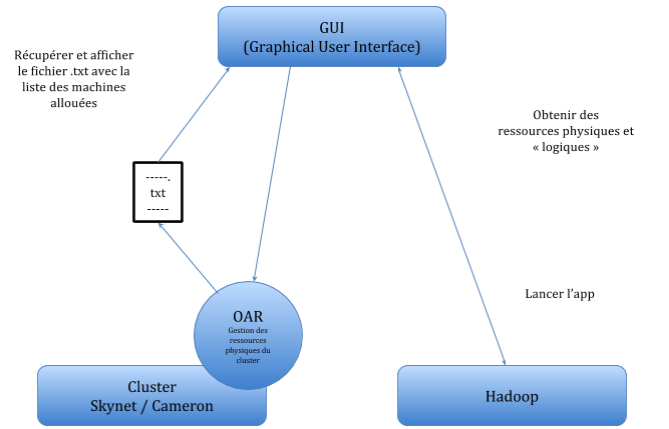
\includegraphics[width=14cm]{images/schema_global.png}
  \caption{Schéma global de fonctionnement de l'application}
  \label{fig:schema_global}
\end{figure}

\par Pour la deuxième partie du projet au cours de la séquence 8, nous utiliserons cette GUI (en anglais \emph{Graphic User Interface}) afin de lancer des applications Hadoop. Pour de plus amples explications concernant l'environnement Hadoop, vous vous référerez au rapport le traitant.
\par Par ailleurs, toutes les requêtes auprès des clusters de Supélec nécessitent des accès sur nos comptes. Accès dont nous avons bénéficié pour nous familiariser avec \emph{OAR}.

\subsection{Architecture du serveur de Supélec}
\label{sec:archi-serveur-supelec}

\par Avant toute chose, il est indispensable de comprendre l'architecture des serveurs de Supélec. Ce serveur est composé de deux machines frontales : \emph{ghome} et \emph{term2} (pour \emph{Terminator 2}). La figure \ref{fig:archi_serveur} reprend cette architecture. Tout utilisateur ayant les droits d'accès au serveur doit impérativement se connecter à la machine \emph{ghome} avant de se connecter à \emph{term2} à travers laquelle il pourra allouer des noeuds grâce à l'environnement \emph{OAR} au sein des clusters \emph{Skynet}, \emph{Cameron} et \emph{InterCel}. Cependant, si l'utilisateur est connecté au réseau de Supélec, l'identification auprès de \emph{term2} est suffisante. Dans le cas échéant il devra nécessairement passer par \emph{ghome}.
\par À titre d'information, \emph{OAR} gère aussi les ressources du cluster \emph{Scooby}. Ce cluster n'est pas utilisé au cours de notre projet.

\begin{figure}[h!]
  \centering
  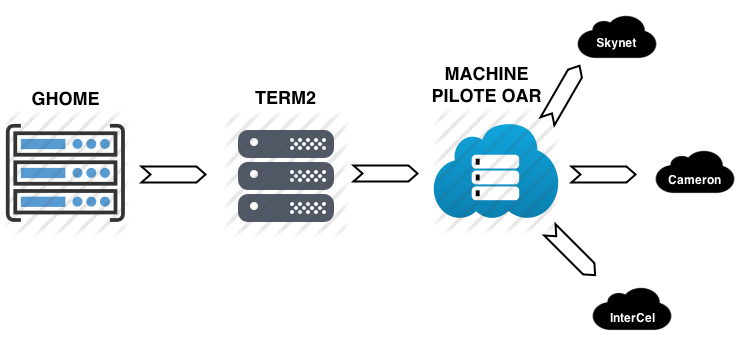
\includegraphics[width=14cm]{images/archi_serveur_supelec.png}
  \caption{Architecture des serveurs de Supélec}
  \label{fig:archi_serveur}
\end{figure}

\subsection{Le diagramme \emph{use case}}
\label{sec:le-diagramme-use}

\par La figure \ref{fig:use_case} donne le diagramme \emph{use case} du projet. Plusieurs scénarios peuvent être répertoriés :

\begin{itemize}
\item \emph{S’identifier};
\item \emph{Créer un job (Allocation de nœuds)};
\item \emph{Tuer le job};
\item \emph{Exécuter des codes Hadoop};
\end{itemize}

\begin{figure}[h!]
  \centering
  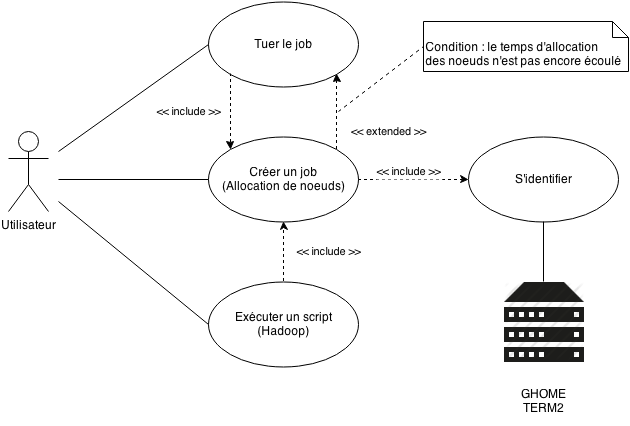
\includegraphics[width=14cm]{images/use_case.png}
  \caption{Use case}
  \label{fig:use_case}
\end{figure}

\paragraph{Scénario \emph{«S’identifier»}}
\par Compte tenu des remarques du paragraphe \vref{sec:archi-serveur-supelec}, il est à rajouter que l'identification préalable auprès de \emph{ghome} n'étant pas gênante pour la suite de l'identification bien que ce dernier soit connecté au réseau de Supélec, nous avons décidé, par souci de praticité, de toujours identifier l'utilisateur auprès de \emph{ghome} puis de \emph{term2}.
\par Cette étape consiste à vérifier la validité du nom ainsi que du mot de passe de l’utilisateur.

\paragraph{Scénario \emph{«Créer un job (Allocation de nœuds)»}}
\label{sec:scenario-creer-un}
\par Après identification, l’utilisateur sera en mesure de créer un job, i.e. d’allouer des nœuds de calcul. Il renseignera donc le nombre de nœuds et le temps d’allocation souhaités. Deux cas de figure se présentent à l'utilisateur. Après la création d’un job, si le temps d’allocation est écoulé le job est automatiquement tué. Dans le cas contraire, l’utilisateur pourra interagir avec la GUI afin de renouveler son job en mettant fin au précédent.

\paragraph{Scénario \emph{«Tuer le job»}}
\label{sec:scenario-tuer-le}
\par Ce scénario n’est évidemment possible que lorsqu’un job a été au préalable créé et que l’utilisateur est connecté au serveur. 

\paragraph{Scénario \emph{«Exécuter un script (Hadoop)»}}
\label{sec:scenario-executer-un}
\par Ce scénario sera abordé dans la deuxième partie du projet se déroulant au cours de la séquence 8.


\subsection{Cahier des charges}
\label{sec:cahier-des-charges}

\par Trois grandes parties composent le cahier des charges.

\subsubsection{Points essentiels}
\label{sec:points-essentiels}

\par La phase d'analyse des différents scénarios a permis d'aboutir à trois points essentiels pour le projet. D’abord nous créerons une IU (Interface Utilisateur) de connexion aux serveurs à travers laquelle il sera possible de spécifier le nom de la machine, le nom de l'utilisateur et son mot de passe.
Ensuite, on créera une deuxième IU d’allocation des nœuds ou seront spécifiés le nombre de nœuds, leur temps d’allocation ainsi que le mode d’allocation (on choisit par défaut le mode interactif).
Enfin, un fichier .txt contenant la description des nœuds alloués devra être récupéré.

\begin{figure}[h!]
  \centering
  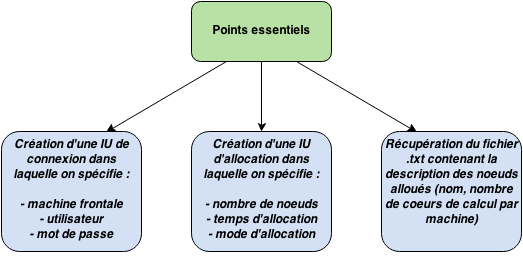
\includegraphics[width=12cm]{images/points_essentiels.png}
  \caption{Cahier des charges : les points essentiels}
  \label{fig:pts_essentiels}
\end{figure}


\subsubsection{Points souhaités}
\label{sec:points-souhaites}

\par Parmi les options fortement souhaitées, l’IU d’allocation devra comporter une zone de texte où sera affiché le temps d’allocation des nœuds en temps réel ainsi que les noms des machines allouées. En outre, le fichier .txt devra être redirigé vers cette zone de texte.

\begin{figure}[h!]
  \centering
  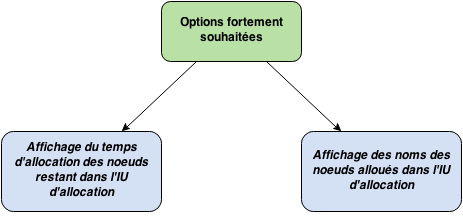
\includegraphics[width=11cm]{images/points_souhaites.png}
  \caption{Cahier des charges : les options fortement souhaitées}
  \label{fig:pts_souhaites}
\end{figure}

\subsubsection{Points optionnels}
\label{sec:points-optionnels}

\par Nous avons retenu trois développements optionnels. Leur réalisation est conditionnée par l’état d’avancement du projet (priorité aux points essentiels et aux options fortement souhaitées) et de leur faisabilité technique.
\par Le premier consiste à obtenir un état des lieux du serveur, i.e. à recenser les ressources physiques disponibles lors de la connexion. L’idée étant dans une deuxième partie de donner à l’utilisateur la possibilité de choisir entre les différents clusters les machines avec lesquelles il désire travailler. En effet, selon que l’on se trouve sur le cluster Skynet, Cameron ou InterCel, les machines ne possèdent pas les mêmes puissances de calcul.
\par Troisièmement, dans le souci de rendre l’expérience utilisateur la plus agréable possible, un design épuré serait fort appréciable. Bien entendu, ce point sera abordé uniquement si tous les précédents points ont été réalisés et validés les tests.

\begin{figure}[h!]
  \centering
  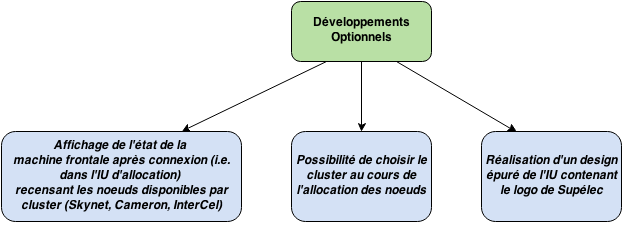
\includegraphics[width=14cm]{images/points_optionnels.png}
  \caption{Cahier des charges : les développements optionnels}
  \label{fig:pts_optionnels}
\end{figure}



%%% Local Variables: 
%%% mode: latex
%%% TeX-master: "CompteRendu"
%%% End: 


% Plan de test

\section{Plan de test}
\label{sec:plan-de-test}

\par L'application devra valider plusieurs tests regroupés sous trois catégories : Affichage, Connexion et Fonctionnalités.

\subsection{Affichage}
\label{sec:affichage}

\par La Boîte connexion MF correspond à l'IU exécutée lors du lancement de l'application. La Boîte OAR quant à elle est l'IU exécutée lorsque la connexion à \emph{term2} est valide.

\begin{table}[h!]
  \centering
  \begin{tabular}[h!]{|c|c|p{10cm}|}
    \hline \\
    1 & Boîte connexion MF & La boîte de connexion à la machine frontale doit s'afficher au lancement du programme. \\
    2 & Boîte connexion MF & La boîte de connexion à la machine frontale doit disparaître lors de l'appuie sur le bouton connexion, avec une adresse machine frontale, un login et un mot de passe valides.\\
    3 & Boîte OAR & La boîte OAR doit s'afficher après une connexion réussie et en même temps que la boîte de connexion MF disparaît. \\
    4 & Boîte OAR & La boîte OAR doit afficher deux champs de saisie, 3 boutons (Tuer le job actif, Allouer les noeuds, Infos sur le job actif), et une zone de texte à hauteur variable. \\
    5 & Boîte OAR & La zone de texte de la boîte OAR doit afficher initialement le message d'accueil du \emph{shell} distant auquel l'interface est connectée. \\

    \hline    
  \end{tabular}
  \caption{Liste des tests d'affichage à valider}
  \label{tab:tests_affichage}
\end{table}

\subsection{Connexion}
\label{sec:connexion}

\par Ce type de tests permettent de valider la connexion aux machines \emph{ghome} et \emph{term2} via l'impression dans la console Java d'un message.

\begin{table}[h!]
  \centering
  \begin{tabular}[h!]{|c|c|p{10cm}|}
\hline \\
    6 & Connexion à \emph{ghome} & Affichage dans la console "Connecté à ghome.metz.supelec.fr sous le port 22"\\
    7 & Connexion à \emph{term2} & Affichage dans la console "Connecté à term2.metz.supelec.fr sous le port xx"\\
\hline
  \end{tabular}
  \caption{Liste des tests de connexion à valider}
  \label{tab:tests_connexion}
\end{table}

\subsection{Fonctionnalités}
\label{sec:fonctions}

\par Dans cette catégorie nous retrouvons les tests concernant les fonctions effectuées par les divers boutons.

\begin{table}[h!]
  \centering
  \begin{tabular}[h!]{|c|p{3cm}|p{10cm}|}
\hline \\
    8 & Bouton "Connexion" & Avec un login et un mot de passe corrects fait disparaître la fenêtre de connexion et affiche la fenêtre d'allocation des noeuds.\\
    9 & Bouton "Allouer des noeuds" & Affiche dans la zone de texte la réponse du \emph{shell} distant à la commande "oarsub" envoyée grâce au clic sur le bouton.\\
    10 & Bouton "Tuer le job actif" & Affiche dans la zone de texte la réponse du \emph{shell} distant à la commande "oardel" envoyée grâce au clic sur le bouton.\\
    11 & Bouton "Infos sur le job actif" & Affiche dans la zone de texte des informations relatives au job en cours d'execution.\\
\hline
  \end{tabular}
  \caption{Liste des tests de connexion à remplir}
  \label{tab:tests_connexion}
\end{table}

%%% Local Variables: 
%%% mode: latex
%%% TeX-master: "CompteRendu"
%%% End: 


% Dossier de conception
\section{Dossier de conception}

\subsection{Diagramme de classes}
\label{sec:diagramme-de-classes}

\begin{figure}[h!]
  \centerline{
  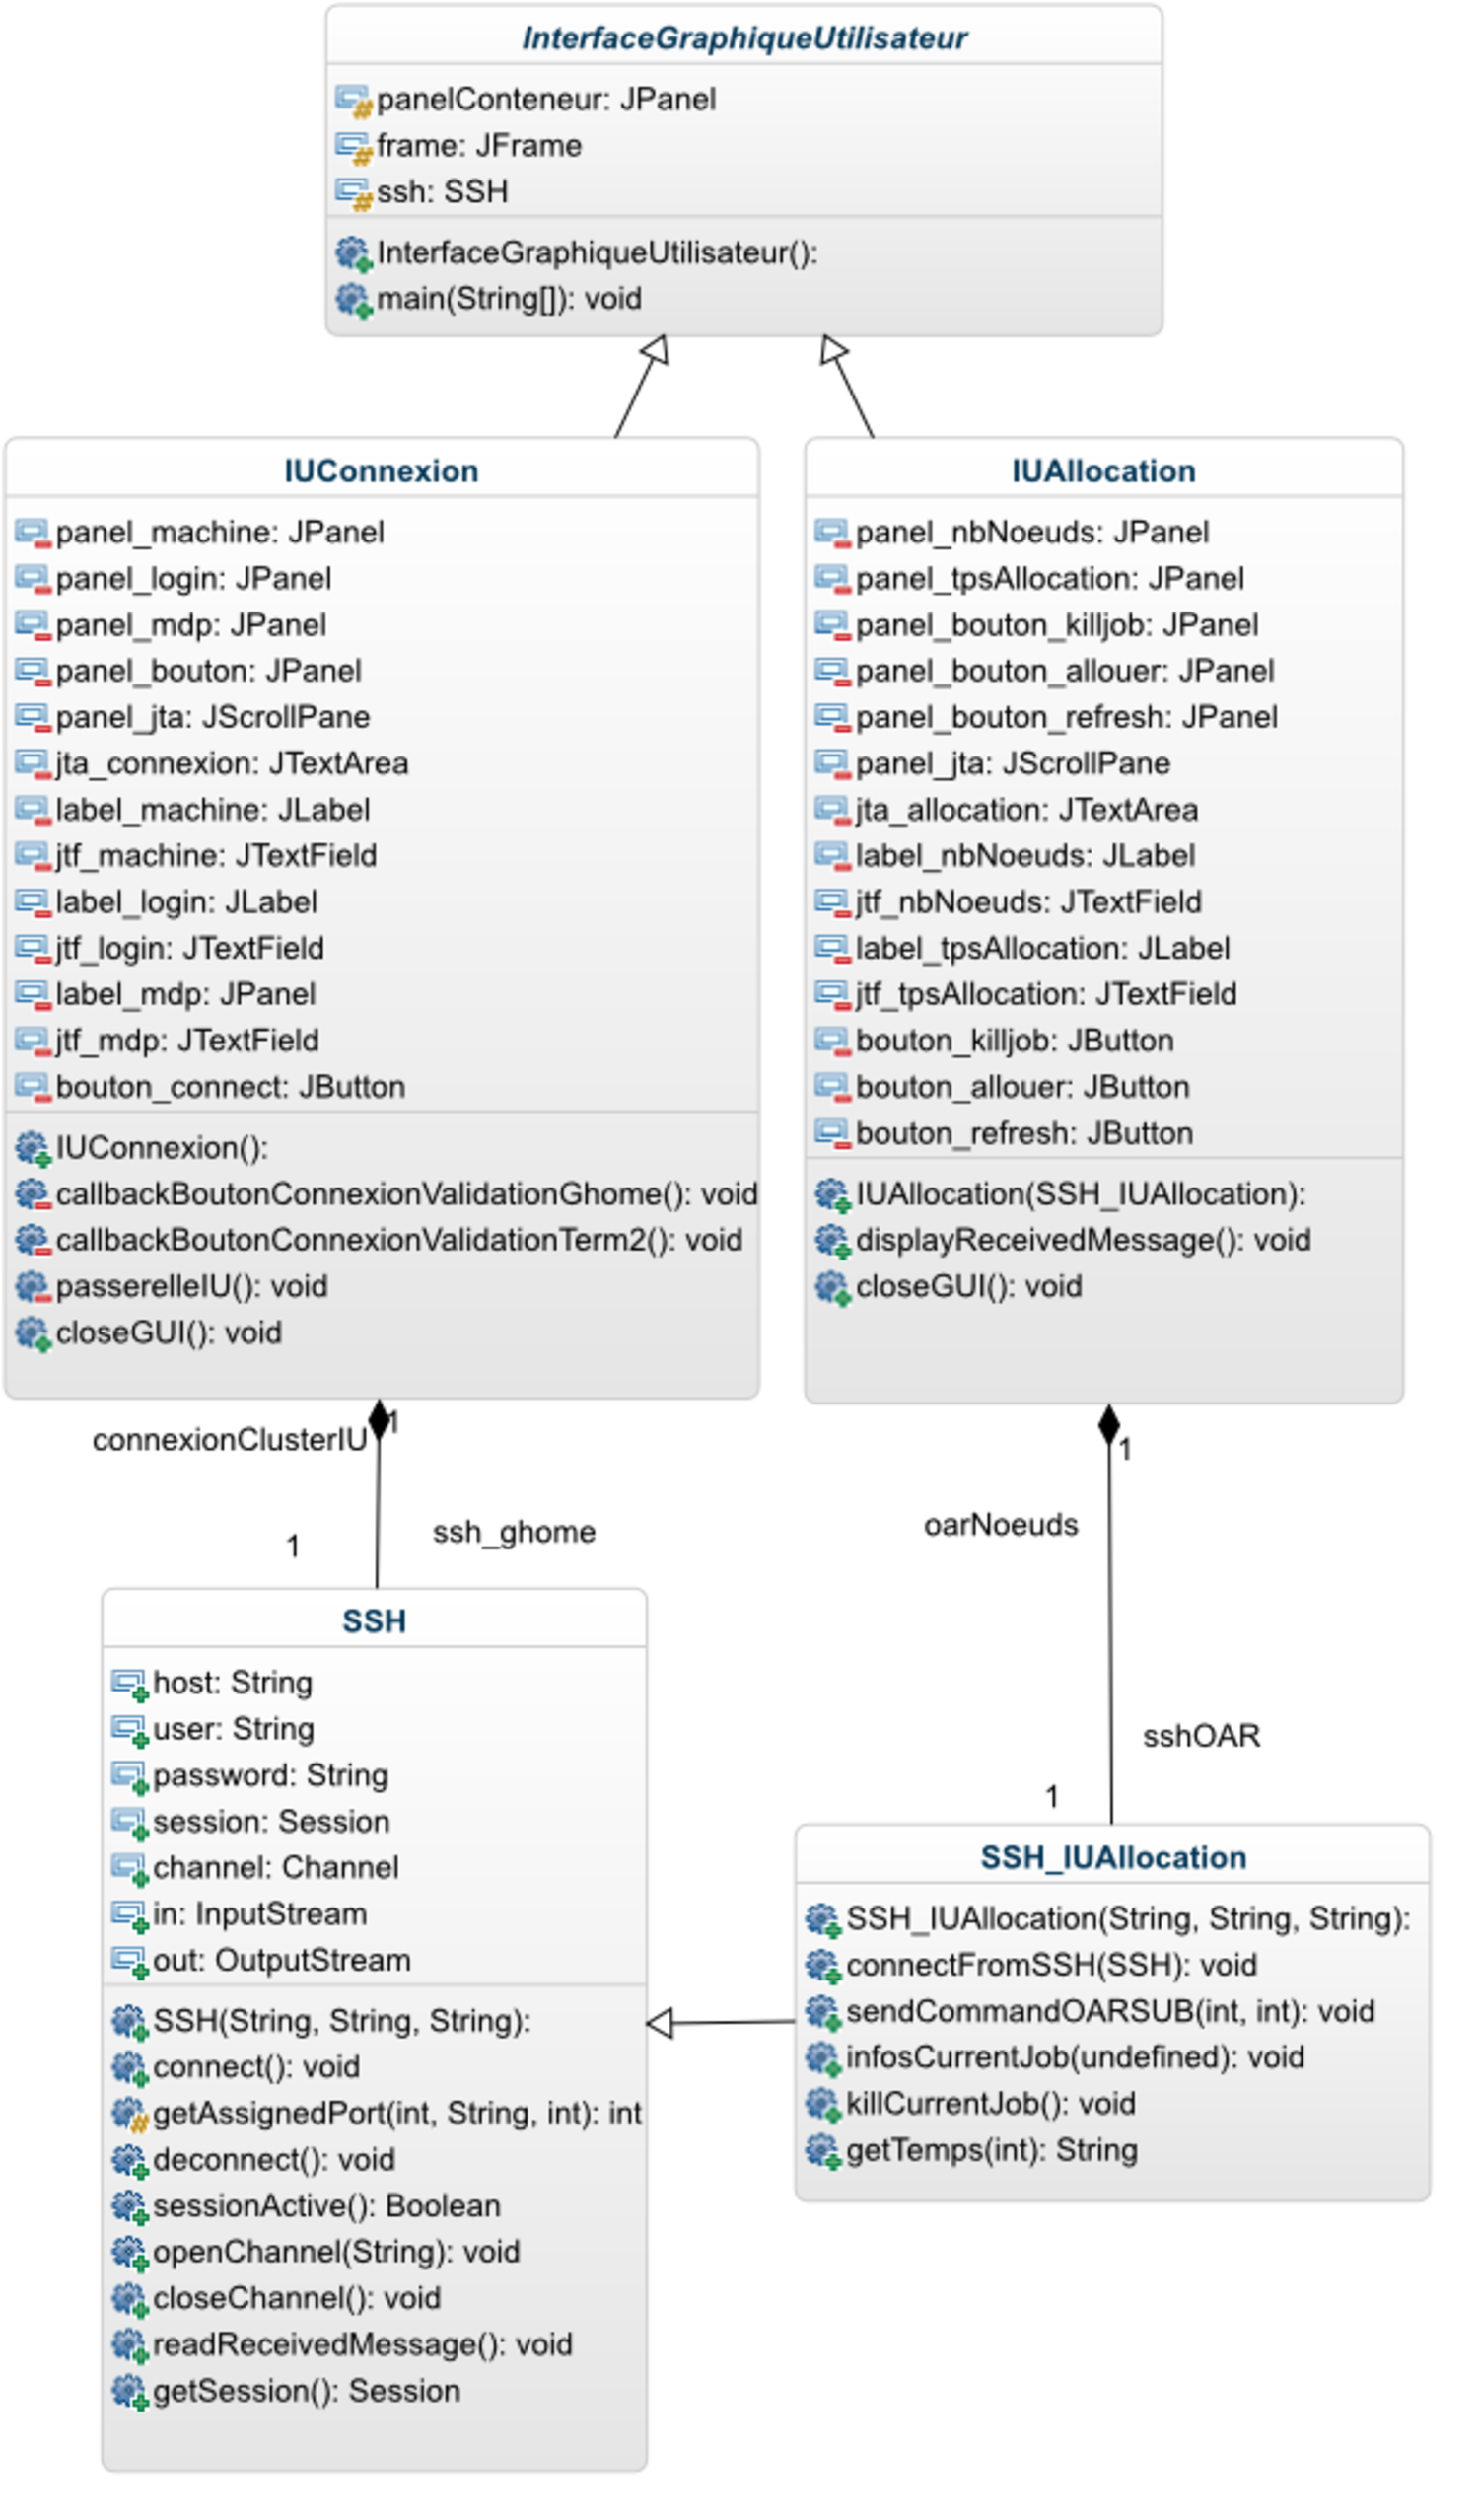
\includegraphics[width=18cm]{images/diagramme_classes.png}}
  \caption{Diagramme des classes}
  \label{fig:diag_classes}
\end{figure}

\subsection{Diagramme de séquence}
\label{sec:diagr-de-sequ}

\begin{figure}[h!]
  \centering
  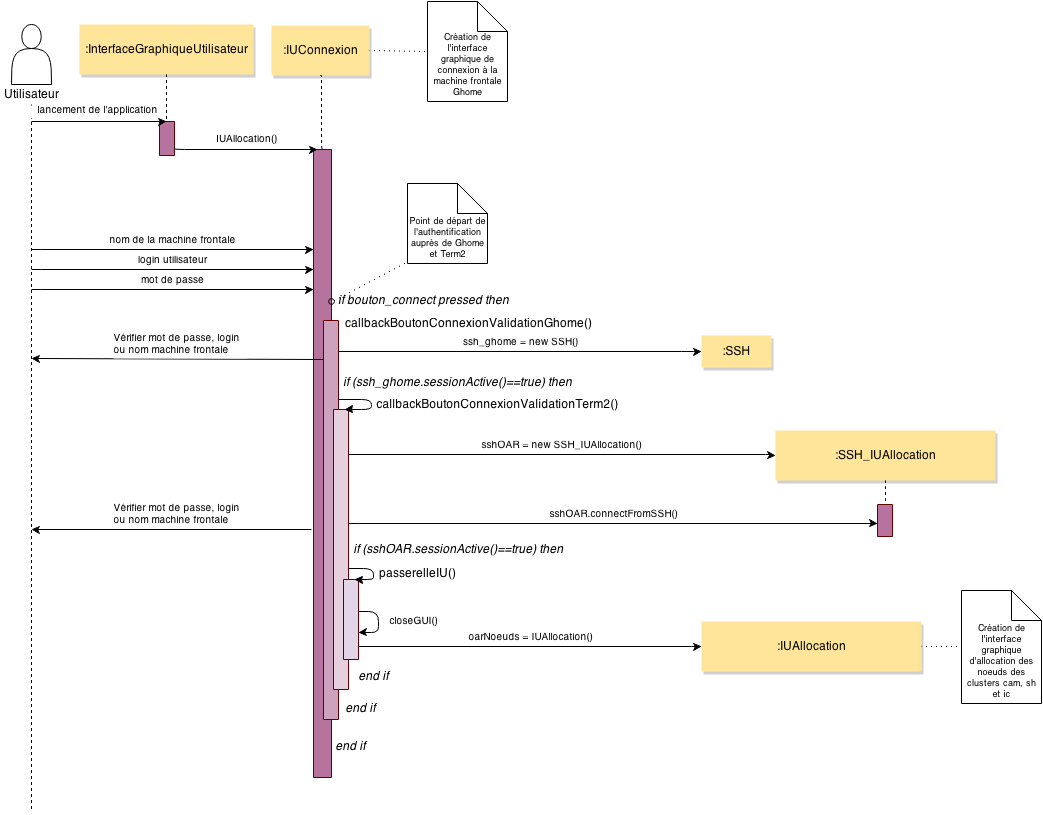
\includegraphics[width=16cm]{images/diagramme_sequence.png}
  \caption{Diagramme de séquence}
  \label{fig:diag_seq}
\end{figure}

\par La figure \ref{fig:diag_seq} donne le diagramme de séquence du scénario «Créer un job».  Tout d'abord, au lancement de l’application par l’utilisateur, l’IU de connexion s’affiche. L’utilisateur est en mesure de renseigner la machine sur laquelle il souhaite se logger, son nom d’utilisateur ainsi que son mot de passe. Lorsque les champs ont été convenablement remplis, l’appui sur le bouton de connexion lance le processus d’identification auprès des serveurs.
\par Une première session ssh est créée dans le serveur GHOME à partir de laquelle, sous condition qu’elle soit active, est créée une deuxième session ssh dans le serveur \texttt{TERM2}. S’il est impossible d’ouvrir une des deux sessions, alors un message d’erreur est renvoyé à l’utilisateur lui demandant de remplir à nouveau les champs. Dans le cas contraire, l’IU de connexion laisse sa place à l’IU d’allocation et le channel de type shell est créé afin d’envoyer les commandes au serveur.
\par L’utilisateur est désormais en mesure de remplir les champs «Nombre de nœuds» et «Temps d’allocation (en min)». L’appui sur le bouton allouer permet d’exécuter la commande ssh. Pour ce faire, plusieurs étapes sont nécessaires. Tout d’abord, les données rentrées par l’utilisateur doivent être traitées et mises sous forme d’une commande shell. La méthode \texttt{sendCommandOARSUB(nbNoeuds, tpsAllocation)} réalise cela en faisant appel à la méthode \texttt{getTemps(int)} afin de mettre sous forme xx:xx:xx heure:minutes:secondes) le temps d’allocation donné en minutes. La commande shell est créée et envoyée via le channel préalablement ouvert.
\par Une fois la commande shell envoyée, la méthode \texttt{readReceivedMessage()} se charge de rediriger vers l’utilisateur, à travers la \texttt{JTextArea} intégrée dans l’IU d’allocation, les données  renvoyées par le serveur. Ces données comprennent, conformément au cahier des charges la liste de nœuds alloués ainsi que les données décrivant l’état de création du job. 
\par Le rafraîchissement de la lecture des données en input du channel, donc provenant du serveur, est assuré par un objet de type Timer ayant pour but toutes les demi secondes de prendre la main afin de tester la présence de données en input. Les données retournées par le serveur semblent donc provenir en continu, sans que l'écoute ne monopolise le thread EDT.
\par Deux cas de figure se présentent à nous désormais concernant le scénario «Tuer le job». Soit le temps d’allocation est écoulé et dans ce cas le job est tué automatiquement par le serveur. Dans ce cas de figure le serveur se charge de reprendre les nœuds qu’il avait alloués. Donc aucune méthode java n’est nécessaire. 
\par Soit l’utilisateur a réalisé une mauvaise manipulation et n’a pas alloué le bon nombre de nœuds ou les a alloués pour une durée trop courte/trop longue (cf. scénario «Tuer le job»). Ici, l’utilisateur aura la possibilité de tuer le job afin d’en créer un nouveau à l’aide du bouton tuer qui appel la méthode \texttt{killCurrentJob()}. Cette méthode va tout simplement construire et envoyer la commande shell permettant de tuer le job courant en allant chercher au sein des variables d’environnement générées par OAR lors de la création du job son identifiant. Ceci évitera par exemple de tuer le job de quelqu’un d’autre.

\subsection{Fonctionnement de Swing}
\label{sec:fonct-de-swing}

AWT (Abstract Windowing Toolkit) est la bibliothèque graphique pour Java introduites dès ses premières versions. Depuis, d’autres API Graphiques ont vu le jour comme Swing, SWT et JFace qui permettent d’améliorer les performances (par exemple la rapidité de la gestion des évènements). Notre projet utilise la bibliothèque Swing, il nous semble par conséquent indispensable de comprendre son fonctionnement.
Swing est une des API Graphique les plus utilisées actuellement et très complexe. Elle est construite à partir de AWT. La majeure différence entre ces deux toolkit, outre leur API et leurs fonctionnalités, réside dans leur nature. En effet, AWT est dit heavyweight (ou lourd) tandis que Swing est dit lightweight (ou léger). Le premier terme désigne le fait que le toolkit est lié directement aux composants natifs nécessaires à l’affichage des applications graphiques alors que le deuxième prend complètement en charge la gestion des composants en les dessinant en pur Java.
Malgré ce degré d’abstraction vis-à-vis du OS, Swing nécessite AWT pour fonctionner. En outre, il utilise son système d’acheminement des évènements qui est la source des problèmes de performances. En effet, toute application Swing est composée de trois threads.
Le premier correspond au main application thread chargé de lancer la méthode main. Le deuxième est le toolkit thread qui a pour but de recevoir les évènements du OS (Ex: appui sur une touche du clavier, clic) et de les transmettre au event dispatching thread ou plus communément appelé EDT. Ce dernier thread est le plus important car il est chargé de répartir les évènements reçus vers les composants concernés et d’appeler les méthodes d’affichage.
Tâchons de mieux comprendre le trio de threads à travers un exemple. Supposons que nous ayons un JTextField et que l’on appuie sur la touche 7. Cet événement est reçu par le « toolkit thread » et traité par l’EDT qui met à jour l’affichage du JTextField en invoquant les méthodes nécessaires de l’IU.
Les applications développées avec la bibliothèque Swing sont réputées pour être lentes du fait que tous les évènements sont traités par un seul et même thread. On comprend très vite l’intérêt d’un traitement en parallèle avec l’intervention de plusieurs threads. Le fonctionnement de l’EDT est similaire à celui d’une file d’attente. Toutes les opérations s’enchaînant successivement, il y a risque de ralentissement de l’exécution d’une opération à cause d’une opération lente. Bien qu’il soit possible que les interfaces graphiques soient peu réactives avec le toolkit Swing, cette bibliothèque ne souffre en aucun cas de mauvaises performances car la compréhension de son fonctionnement (trio de threads) permet de réaliser des interfaces réactives à l’aide de plusieurs modèles de gestion des threads qui permettent de rendre l’API « thread safe » (i.e. que les méthodes peuvent être exécutées par plusieurs threads s’exécutant en même temps).

\par Nous avons été bloqués un bon moment à cause d'une mauvaise gestion du thread EDT. En effet, l'utilisation d'une boucle infinie pour vérifier le contenu du buffer \texttt{in} monopolisait le thread EDT, empêchant toute autre action, notamment la mise à jour du contenu des fenêtres graphiques, et également la gestion des autres événements. L'utilisation d'un Timer, qui execute à intervalles réguliers un morceau de code logé dans un objet \texttt{Runnable}, a permis de résoudre le problème, tout en gardant une réactivité équivalente.

%%% Local Variables: 
%%% mode: latex
%%% TeX-master: "CompteRendu"
%%% End: 


% Vérification des tests



% Dossier user guide
\section{Partie \emph{user guide}}
\label{sec:user-guide}

\par L’interface graphique est très facile de prise en main.
\par Une bonne utilisation de l'application passe naturellement par un tutoriel expliquant les diverses fonctionnalités de cette dernière.

\paragraph{Lancement de l'application et connexion au serveur Supélec}
\label{sec:lancement_app}

\par Au lancement de l’application, l’IU de connexion figure \ref{fig:iucon_launch} se lance.

\begin{figure}[h!]
  \centering
  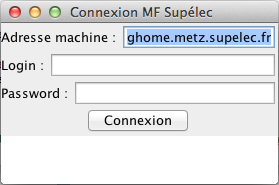
\includegraphics[width=6cm]{images/iuconnexion_launch.png}
  \caption{IU de connexion au lancement de l'application}
  \label{fig:iucon_launch}
\end{figure}

\par L’utilisateur doit renseigner l’adresse de la machine frontale sur laquelle il souhaite se connecter (la valeur par défaut est ghome.metz.supelec.fr), son login ainsi que son mot de passe comme réalisé à la figure \ref{fig:iucon_connect}.

\begin{figure}[h!]
  \centering
  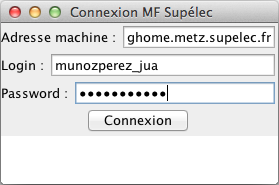
\includegraphics[width=6cm]{images/iuconnexion_connect.png}
  \caption{IU de connexion au lancement de l'application}
  \label{fig:iucon_connect}
\end{figure}

\par L’appui sur le bouton \emph{Connexion} lance l’identification auprès du serveur Supélec. Si l'authentification est valide, l'IU de connexion se ferme et l'IU d'allocation apparaît.

\paragraph{Allocation de noeuds : création d'un job}

\par La figure \ref{fig:iualloc_launch} représente l'IU d'allocation.

\begin{figure}[h!]
  \centering
  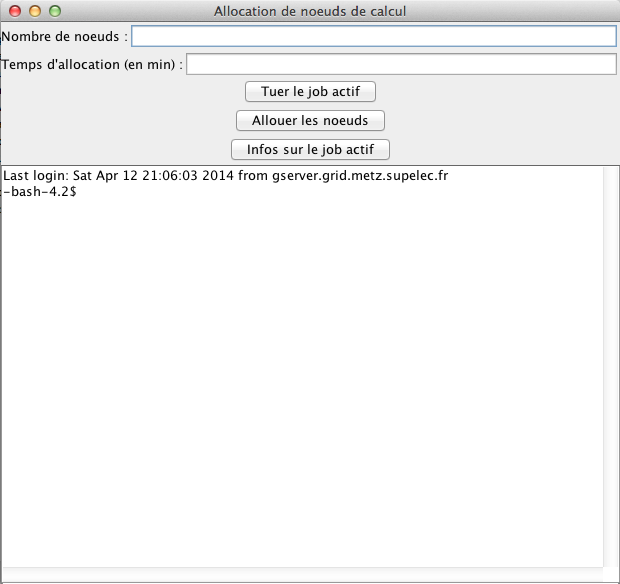
\includegraphics[width=11cm]{images/iuallocation_launch.png}
  \caption{IU d'allocation après validation de l'authentification}
  \label{fig:iualloc_launch}
\end{figure}

\par À ce stade il est désormais possible d'allouer des noeuds de calcul. Pour ce faire, l'utilisateur doit renseigner le nombre de noeuds souhaités (un entier naturel) ainsi que le temps d'allocations (en minutes). Après appui sur le bouton \emph{Allouer des noeuds}, l'IU d'allocation ressemble à la figure \ref{fig:iualloc_nodes}.

\begin{figure}[h!]
  \centering
  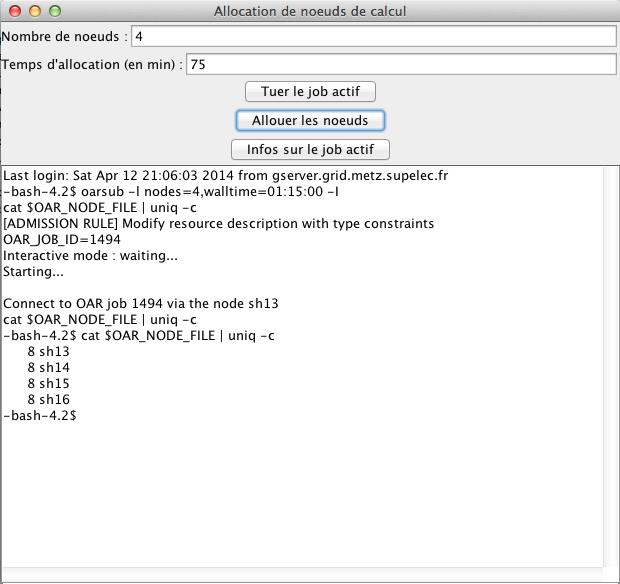
\includegraphics[width=11cm]{images/iuallocation_ask_nodes.png}
  \caption{IU d'allocation : allocation de noeuds}
  \label{fig:iualloc_nodes}
\end{figure}

\par Nous pouvons voir que le job correspondant à notre requête est le job numéro 1494. La machine de référence est le nœud sh13 (machine du cluster Skynet). Les nœuds qui nous sont alloués pour une durée de 75 minutes sont sh13 (8), sh14 (8), sh15 (8) et sh16 (8). Le nombre entre parenthèses correspond au nombre de cœurs processeurs que possède la machine. D’un cluster à l’autre il se peut que ce nombre varie. Pour indication, les machines du cluster Cameron possèdent 6 cœurs alors que celles d’InterCel n’en possèdent que 2.

\paragraph{Informations sur le job}
\label{sec:info_job}

\par Le job étant actif il est possible d'obtenir des informations sur l'identifiant du job, le temps d'allocation restant, les ressources qui ont été assignées et bien d'autres.
\par L'appui sur le bouton \emph{Infos sur le job actif} nous renvoie sur la fenêtre le message ci dessous.

\begin{verbatim}
-bash-4.2$ oarstat -fj $OAR_JOB_ID
Job_Id: 1494
    job_array_id = 1494
    job_array_index = 1
    name = 
    project = default
    owner = munozperez_jua
    state = Running
    wanted_resources = -l "{type = 'default'}/network_address=4,walltime=1:15:0" 
    types = 
    dependencies = 
    assigned_resources = 105+106+107+108+109+110+111+112+113+114+115+
116+117+118+119+120+121+122+123+124+125+126+127+128+129+130+131+132+
133+134+135+136
    assigned_hostnames = sh13+sh14+sh15+sh16
    queue = default
    command = 
    launchingDirectory = /usr/users/promo2015/munozperez_jua
    stdout_file = OAR.1494.stdout
    stderr_file = OAR.1494.stderr
    jobType = INTERACTIVE
    properties = desktop_computing = 'NO'
    reservation = None
    walltime = 1:15:0
    submissionTime = 2014-04-12 21:53:53
    startTime = 2014-04-12 21:53:54
    cpuset_name = munozperez_jua_1494
    initial_request = oarsub -l nodes=4,walltime=01:15:00 -I
    message = R=32,W=1:15:0,J=I (Karma=0.815)
    scheduledStart = 2014-04-12 21:53:54
    resubmit_job_id = 0
    events = 
\end{verbatim}

\par Il sera possible à tout moment, tant qu'il y a un job actif, de suivre l'évolution du job. 

\paragraph{Tuer le job}
\label{sec:tuer_job}

\par Si jamais l'utilisateur s'est trompé dans le nombre de noeuds ou le temps d'allocation lors de la création de son job, il est possible de revenir en arrière en tuant ledit job. Pour ce faire, il suffit d'appuyer sur le bouton \emph{Tuer le job actif}.
\par La figure \ref{fig:iualloc_kill} montre le message renvoyé par le serveur après exécution de la commande. 

\begin{figure}[h!]
  \centering
  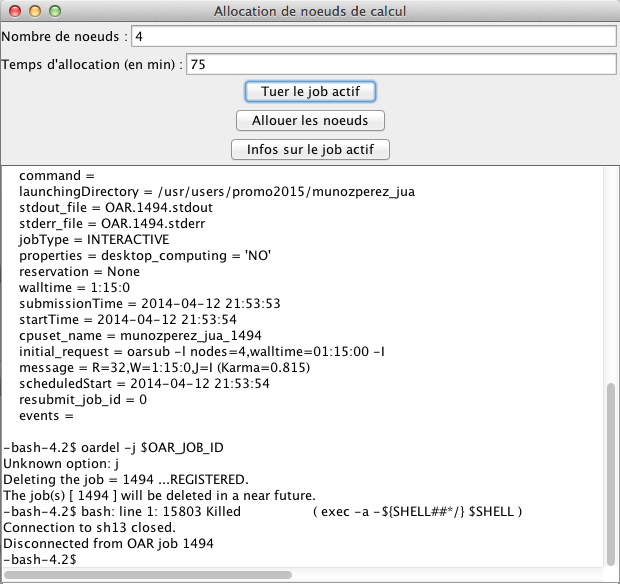
\includegraphics[width=11cm]{images/iuallocation_kill_job.png}
  \caption{IU d'allocation : tuer le job}
  \label{fig:iualloc_kill}
\end{figure}

\par Éliminer le job actif 1494 consiste tout simplement pour \emph{OAR} à fermer la connexion à la machine de référence, ici sh13.
\par À travers ce tutoriel, nous avons bien vu que l'application implémentée réalise bien les fonctionnalités mentionnées dans les précédentes parties et est très simple d'utilisation.

%%% Local Variables: 
%%% mode: latex
%%% TeX-master: "CompteRendu"
%%% End: 

% Conclusion

\section{Conclusion}
\label{sec:conclusion}

\par Au cours de ce projet, nous avons été amenés à manipuler un certain nombre de concepts. Nous nous sommes donc par conséquent focalisés sur ces notions nouvelles, que nous pensions être la principale difficulté de cette entreprise. Cependant, nous avons rencontré quelques problèmes inattendus, qui se sont révélés plus compliqués à comprendre et à résoudre que nous ne l'avions prévu. \par En effet, la réalisation de l'interface graphique nous avait paru plutôt simple, et ne devait pas nécessiter un approfondissement important. Malheureusement, l'utilisation \og exotique\fg{} que nous en avons fait nous aura obligés à comprendre comment elle est structurée, comment elle fonctionne.
\par En définitive, le programme fonctionne et remplit le cahier des charges, et peut aisément être amélioré maintenant que son squelette est établi et fonctionnel.


%%% Local Variables: 
%%% mode: latex
%%% TeX-master: "CompteRendu"
%%% End: 


\nocite{github}
\nocite{marseille-oar}
\nocite{vialle:oar}
\nocite{git:eclipse}
\nocite{jsch:website}
\nocite{ssh:connection}
\nocite{run:shell:commands}
\nocite{javadoc:jsch}
\nocite{ssh:beanizer}
\nocite{jsch:manual}
\nocite{ssh:guide}
\nocite{oar:userguide}
\nocite{sdz:layout}
\nocite{threads:developpez}
\nocite{oar2}
\nocite{git}
\nocite{shell}

\null
\newpage
\printbibliography

\end{document}
